% A LaTeX template for EXECUTIVE SUMMARY of the MSc Thesis submissions to 
% Politecnico di Milano (PoliMi) - School of Industrial and Information Engineering
%
% S. Bonetti, A. Gruttadauria, G. Mescolini, A. Zingaro
% e-mail: template-tesi-ingind@polimi.it
%
% Last Revision: October 2021
%
% Copyright 2021 Politecnico di Milano, Italy. NC-BY

\documentclass[11pt,a4paper,twocolumn]{article}

%------------------------------------------------------------------------------
%	REQUIRED PACKAGES AND  CONFIGURATIONS
%------------------------------------------------------------------------------
% PACKAGES FOR TITLES
\usepackage{titlesec}
\usepackage{color}

% PACKAGES FOR LANGUAGE AND FONT
\usepackage[utf8]{inputenc}
\usepackage[english]{babel}
\usepackage[T1]{fontenc} % Font encoding

% PACKAGES FOR IMAGES
\usepackage{graphicx}
\graphicspath{{Images/}} % Path for images' folder
\usepackage{eso-pic} % For the background picture on the title page
\usepackage{subfig} % Numbered and caption subfigures using \subfloat
\usepackage{caption} % Coloured captions
\usepackage{transparent}

% STANDARD MATH PACKAGES
\usepackage{amsmath}
\usepackage{amsthm}
\usepackage{bm}
\usepackage[overload]{empheq}  % For braced-style systems of equations

% PACKAGES FOR TABLES
\usepackage{tabularx}
\usepackage{longtable} % tables that can span several pages
\usepackage{colortbl}

% PACKAGES FOR ALGORITHMS (PSEUDO-CODE)
\usepackage{algorithm}
\usepackage{algorithmic}

% PACKAGES FOR REFERENCES & BIBLIOGRAPHY
\usepackage[colorlinks=true,linkcolor=black,anchorcolor=black,citecolor=black,filecolor=black,menucolor=black,runcolor=black,urlcolor=black]{hyperref} % Adds clickable links at references
\usepackage{cleveref}
\usepackage[square, numbers, sort&compress]{natbib} % Square brackets, citing references with numbers, citations sorted by appearance in the text and compressed
\bibliographystyle{plain} % You may use a different style adapted to your field

% PACKAGES FOR THE APPENDIX
\usepackage{appendix}

% PACKAGES FOR ITEMIZE & ENUMERATES 
\usepackage{enumitem}

% OTHER PACKAGES
\usepackage{amsthm,thmtools,xcolor} % Coloured "Theorem"
\usepackage{comment} % Comment part of code
\usepackage{fancyhdr} % Fancy headers and footers
\usepackage{lipsum} % Insert dummy text
\usepackage{tcolorbox} % Create coloured boxes (e.g. the one for the key-words)
\usepackage{stfloats} % Correct position of the tables


%-------------------------------------------------------------------------
%	NEW COMMANDS DEFINED
%-------------------------------------------------------------------------
% EXAMPLES OF NEW COMMANDS -> here you see how to define new commands
\newcommand{\bea}{\begin{eqnarray}} % Shortcut for equation arrays
\newcommand{\eea}{\end{eqnarray}}
\newcommand{\e}[1]{\times 10^{#1}}  % Powers of 10 notation
\newcommand{\mathbbm}[1]{\text{\usefont{U}{bbm}{m}{n}#1}} % From mathbbm.sty
\newcommand{\pdev}[2]{\frac{\partial#1}{\partial#2}}
% NB: you can also override some existing commands with the keyword \renewcommand

%----------------------------------------------------------------------------
%	ADD YOUR PACKAGES (be careful of package interaction)
%----------------------------------------------------------------------------

\usepackage{todonotes}
\usepackage{xurl}
\usepackage{subfiles}
\usepackage{siunitx}
\usepackage{csquotes}
\usepackage{svg}
\usepackage{tikz}
\usepackage{listings}
%----------------------------------------------------------------------------
%	ADD YOUR DEFINITIONS AND COMMANDS (be careful of existing commands)
%----------------------------------------------------------------------------
\newcommand{\parspace}{\vspace{7pt}}
\newlist{inlinelist}{enumerate*}{1}
\setlist[inlinelist]{label=(\arabic*)}

% Do not change Configuration_files/config.tex file unless you really know what you are doing. 
% This file ends the configuration procedures (e.g. customizing commands, definition of new commands)
% Configuration package
\usepackage[bottom=2.0cm,top=2.0cm,left=2.0cm,right=2.0cm]{geometry}
\raggedbottom 

% Create color bluePoli (-> manuale grafica coordinata:  https://www.polimi.it/fileadmin/user_upload/il_Politecnico/grafica-coordinata/2015_05_11_46xy_manuale_grafica_coordinata.pdf)
\definecolor{bluePoli}{cmyk}{0.4,0.1,0,0.4}

% Custom theorem environments
\declaretheoremstyle[
  headfont=\color{bluePoli}\normalfont\bfseries,
  bodyfont=\color{black}\normalfont\itshape,
]{colored}

\captionsetup[figure]{labelfont={color=bluePoli}} % Set colour of the captions
\captionsetup[table]{labelfont={color=bluePoli}} % Set colour of the captions
\captionsetup[algorithm]{labelfont={color=bluePoli}} % Set colour of the captions

\theoremstyle{colored}
\newtheorem{theorem}{Theorem}[section]
\newtheorem{proposition}{Proposition}[section]

% Enhances the features of the standard "table" and "tabular" environments.
\newcommand\T{\rule{0pt}{2.6ex}}
\newcommand\B{\rule[-1.2ex]{0pt}{0pt}}

% Algorithm description
\newcounter{algsubstate}
\renewcommand{\thealgsubstate}{\alph{algsubstate}}
\newenvironment{algsubstates}{
    \setcounter{algsubstate}{0}%
    \renewcommand{\STATE}{%
    \stepcounter{algsubstate}%
    \Statex {\small\thealgsubstate:}\space}
    }{}
    
% Custom theorem environment
\newcolumntype{L}[1]{>{\raggedright\let\newline\\\arraybackslash\hspace{0pt}}m{#1}}
\newcolumntype{C}[1]{>{\centering\let\newline\\\arraybackslash\hspace{0pt}}m{#1}}
\newcolumntype{R}[1]{>{\raggedleft\let\newline\\\arraybackslash\hspace{0pt}}m{#1}}

% Custom itemize environment
\setlist[itemize,1]{label=$\bullet$}
\setlist[itemize,2]{label=$\circ$}
\setlist[itemize,3]{label=$-$}
\setlist{nosep}

% Create command for background pic
\newcommand\BackgroundPic{% Adding background picture
	\put(237,365){
	    \parbox[b][\paperheight]{\paperwidth}{%
	    \vfill
		\centering
		\transparent{0.4}
		
\includegraphics[width=0.44\paperwidth]{raggiera_polimi.eps}%
		\vfill}
		}
}

% Set indentation
\setlength\parindent{0pt}

% Custom title commands
\titleformat{\section}
{\color{bluePoli}\normalfont\Large\bfseries}
{\color{bluePoli}\thesection.}{1em}{}
\titlespacing*{\section}
{0pt}{3.3ex}{3.3ex}

\titleformat{\subsection}
{\color{bluePoli}\normalfont\large\bfseries}
{\color{bluePoli}\thesubsection.}{1em}{}
\titlespacing*{\subsection}
{0pt}{3.3ex}{3.3ex}

% Custom headers and footers
\pagestyle{fancy}
\fancyhf{}
      
\fancyfoot{}
\fancyfoot[C]{\thepage} % page
\renewcommand{\headrulewidth}{0mm} % headrule width
\renewcommand{\footrulewidth}{0mm} % footrule width

\makeatletter
\patchcmd{\headrule}{\hrule}{\color{black}\hrule}{}{} % headrule
\patchcmd{\footrule}{\hrule}{\color{black}\hrule}{}{} % footrule
\makeatother

% Insert here the info that will be displayed into your Title page 
% -> title of your work
\renewcommand{\title}{Why can you kill mosquitoes in the dark? \\
    \large Towards solving sound localization with a biologically plausible spiking neural simulation}
% -> author name and surname
\renewcommand{\author}{Paolo Marzolo}
% -> MSc course
\newcommand{\course}{Computer Science and Engineering - Ingegneria Informatica}
% -> advisor name and surname
\newcommand{\advisor}{Prof. Alberto Antonietti}
% IF AND ONLY IF you need to modify the co-supervisors you also have to modify the file Configuration_files/title_page.tex (ONLY where it is marked)
\newcommand{\firstcoadvisor}{Eng. Francesco De Santis} % insert if any otherwise comment
%\newcommand{\secondcoadvisor}{Name Surname} % insert if any otherwise comment
% -> academic year
\newcommand{\YEAR}{2024-2025}

%-------------------------------------------------------------------------
%	BEGIN OF YOUR DOCUMENT
%-------------------------------------------------------------------------
\begin{document}

%-----------------------------------------------------------------------------
% TITLE PAGE
%-----------------------------------------------------------------------------
% Do not change Configuration_files/TitlePage.tex (Modify it IF AND ONLY IF you need to add or delete the Co-advisors)
% This file creates the Title Page of the document
% DO NOT REMOVE SPACES BETWEEN LINES!

\twocolumn[{\begin{@twocolumnfalse}

\AddToShipoutPicture*{\BackgroundPic}

\hspace{-0.6cm}
\includegraphics[width=0.6\textwidth]{logo_polimi_ing_indinf.eps}

\vspace{-1mm}
\fontsize{0.3cm}{0.5cm}\selectfont \bfseries \textsc{\color{bluePoli} Executive Summary of the Thesis}\\

\vspace{-0.2cm}
\Large{\textbf{\color{bluePoli}{\title}}}\\

\vspace{-0.2cm}
\fontsize{0.3cm}{0.5cm}\selectfont \bfseries \textsc{\color{bluePoli} Laurea Magistrale in \course}\\

\vspace{-0.2cm}
\fontsize{0.3cm}{0.5cm} \selectfont \bfseries Author: \textsc{\textbf{\author}}\\

\vspace{-0.4cm}
\fontsize{0.3cm}{0.5cm}\selectfont \bfseries Advisor: \textsc{\textbf{\advisor}}\\

% if only ONE co-advisor is present:
\vspace{-0.4cm}
\fontsize{0.3cm}{0.5cm}\selectfont \bfseries Co-advisor: \textsc{\textbf{\firstcoadvisor}}\\
% if more than one co-advisors are present:
%\vspace{-0.4cm}
%\fontsize{0.3cm}{0.5cm}\selectfont \bfseries Co-advisors: \textsc{\textbf{\firstcoadvisor}}\textsc{\textbf{\secondcoadvisor}}\\

\vspace{-0.4cm}
\fontsize{0.3cm}{0.5cm}\selectfont \bfseries Academic year: \textsc{\textbf{\YEAR}}

\small \normalfont

\vspace{11pt}

\centerline{\rule{1.0\textwidth}{0.4pt}}

\vspace{15pt}
\end{@twocolumnfalse}}]

\thispagestyle{plain} % In order to not show the header in the first page

%-----------------------------------------------------------------------------
% INTRODUCTION
%-----------------------------------------------------------------------------
\section{Introduction}\label{sec:introduction}
The task of sound localization consists of identifying the source position of a sound. Differently from sight and somatosensation (touch), stimulus location is not directly linked to a sensory organ region. Hence, sound source position must be \textit{derived} from the original input; this derivation is based on three main features (\textit{auditory cues}): the differences in time and loudness (\textit{level}) between when a sound reaches each ear, namely the interaural time difference (ITD) and interaural level difference (ILD), and the difference in how a sound gets distorted by the obstacles it encounters along its path (the body, the head and the outer ear), depending on its source location. This work focuses on horizontal (azimuthal) localization, for which only the first two cues are relevant. In the mammalian brain, these cues are generally associated with distinct nuclei in the superior olivary complex (SOC), which respectively show increased sensibility to a single cue: the medial superior olive (MSO) for the ITD, and the lateral superior olive (LSO) for the ILD. Unlike the processing of ILD, the processing of ITDs is less understood. Multiple strategies have been proposed; the most impactful is a model presented by Jeffress in 1948. This model assumes that ITDs are processed by an array of simple coincidence detectors (neurons that respond maximally when the two inputs arrive simultaneously), wired with progressively longer delay lines (based on axonal length) that generate internal delays. Then, the coincidence detector that fires maximally will represent the current ITD, generating an internal map of ITDs. The two structures that power the Jeffress scheme (delay lines and ITD map) were confirmed to exist in the avian brain \cite{grotheMechanismsSoundLocalization2010}. Due to parallel evolution, it is possible that findings obtained in different lineages (birds) may not exist in the mammalian brainstem, and indeed, there is very weak evidence of these structures in mammals. This has pushed research into looking for the alternative mechanism in use in mammals. One such proposal is Myoga's \cite{myogaGlycinergicInhibitionTunes2014}, who focused on the timing of excitatory and inhibitory inputs. The MSO receives four inputs from lower-level nuclei: a pair of inhibition and excitation from each side. The authors found that both sources of inhibition to the MSO can be used to tune its ability to perform coincidence detection, hence changing the ITD value for which the MSO cells will have the maximum response.

\parspace
The first neural step of the auditory pathway are the auditory nerve fibers (ANFs), which receive the signal after it has been elaborated and transduced into a graded potential by the peripheral processing sections. The source transducers (which are the inner hair cells inside the cochlea) only respond to a specific frequency, called the characteristic frequency (CF): this causes the entire neural population to be organized by frequency. The ANFs then converge to two main populations, the spherical bushy cells (SBCs) and globular bushy cells (GBCs). The SBCs are the main source of excitation to the SOC nuclei, while the GBCs, after an additional step to transform the signal from excitatory to inhibitory, provide the main source of inhibition. The LSO receives excitation from the SBCs and inhibition from the contralateral GBCs (mediated by cells of the medial nucleus of the trapezoid body, MNTB); the MSO receives excitation from both sides of SBCs, and inhibition from ipsilateral GBCs (mediated by cells of the lateral nucleus of the trapezoid body, LNTB) and from contralateral GBCs (once again mediated by cells in the MNTB).
We show the complete network, together with the connectivity patterns, the delays and synaptic weights we used, in Figure~\ref{fig:network}.

\begin{figure*}
    \centering
    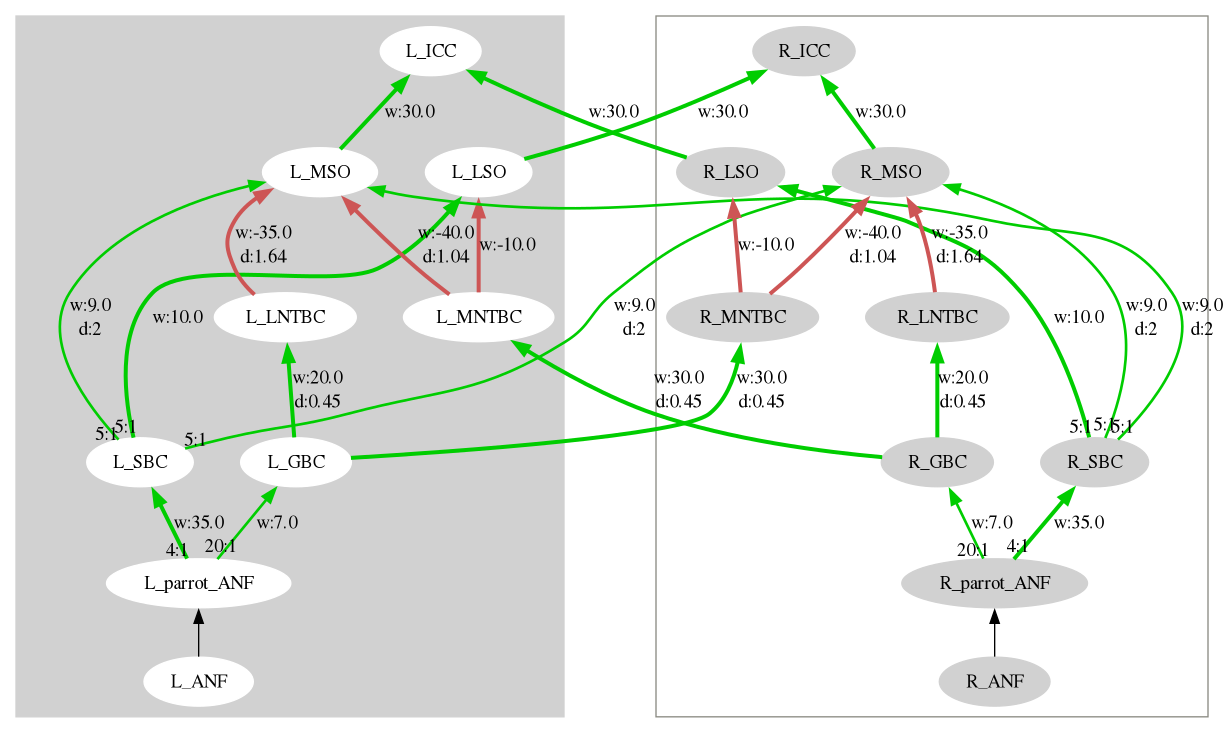
\includegraphics[width=0.9\linewidth]{Images/netvis.png}
    \caption{The complete network, from ANFs to IC. Green connections are excitatory, red are inhibitory. Next to each connection, its synaptic weight and delay. From ANFs and bushy cells, the notation X:Y shows convergence information.}
    \label{fig:network}
\end{figure*}

\parspace

The LSO and MSO then converge to the inferior colliculus (IC). Although the IC comprises three regions - central nucleus, dorsal cortex, and external cortex - the central nucleus (ICC) is the primary region of interest for auditory processing, together with the brachium of the IC. The ICC receives input from both of the SOC nuclei discussed so far, LSO and MSO, in addition to other sources; specifically, each IC receives input from ipsilateral MSO and contralateral LSO. These synapses are mostly excitatory, forming an EE scheme (excitatory-excitatory) \cite{grotheMechanismsSoundLocalization2010}. Cells in the ICC have shown varying properties and classified accordingly: type V units, sensitive to ITDs, type I units, sensitive to ILDs, and type IV units, resembling neurons in the dorsal cochlea nucleus, which processes spectral cues. Evidence for a spatial map has not been found, and some results \cite{sleeAlignmentSoundLocalization2014} suggest that auditory cues may remain more segregated than previously thought. Overall, the literature does not definitively answer whether and how auditory cues are integrated above the SOC.

\parspace
In this work, we create a bioplausible network for auditory localization, with three main steps. First, we mimic biological auditory processing structures to create realistic inputs for a neural simulation, containing both intermediate populations and the two nuclei of interest. Second, we use Myoga's principles to create a plausible MSO that shows increased activity for contralateral sounds, as seen in literature. Finally, we investigate whether this MSO adds information to the LSO for the localization of tones at different frequencies, by creating a synthetic inferior colliculus (the anatomical site of convergence of LSO and MSO) with a simple EE scheme and testing its performance.

\section{Objectives}
Given the state of research around sound localization, this work improves an existing, simplified, neural-only computational model \cite{santisComputationalModelMammalian}, with three main objectives:
\begin{enumerate}
    \item\label{obj:bioplaus} Improve the overall bioplausibility of the existing model by:
    \begin{enumerate}
        \item Implementing peripheral sections at three levels of bioplausibility:
        \begin{inlinelist}
            \item\label{obj:coch-pulse} \textit{Pulse packet}
            \item\label{obj:coch-gamm} \textit{Gammatone-based}
            \item\label{obj:coch-tc} \textit{Tan-Carney realistic mammalian cochlea}
        \end{inlinelist}
        \item Evaluating the effect of these peripheral sections on SOC nuclei (LSO and MSO)
    \end{enumerate}
    \item\label{obj:mso} Use Myoga's principles to produce a contralateral-favoring MSO without the use of dedicated delay lines
    \item\label{obj:icc} Consider an EE (contralateral LSO and ipsilateral MSO) scheme for auditory cue integration above the SOC with a synthesized IC model and quantitatively evaluate it on three metrics:
    \begin{enumerate}
        \item \textit{Zero-degree accuracy}: Since behavioral results show no difference between right and left azimuthal localization accuracy, the center point (zero degrees) should show equal activation in both populations;
        \item \textit{Increased sensitivity around zero}: Just noticeable difference, a metric that shows the lowest detectable degree difference between sounds, is lowest in humans around zero azimuth. Hence, a steeper curve is an improvement;
        \item \textit{Range}: Difference between maximum and minimum total population spike index to maximize the difference in lateralization.
    \end{enumerate}
\end{enumerate}


\section{Methods}
This project was split in two sections: the first focused on increasing the bioplausibility of the peripheral system, and the second one implemented the neural processing. The modeling of the peripheral section, from the sound to the spiking output of ANFs, was implemented using Brian2Hears \cite{fontaineBrianHearsOnline2011}, an extension to Brian 2 \cite{stimbergBrian2Intuitive2019}, a widely used open-source spiking neural network simulator. The modeling of the central nervous system was developed using NEST \cite{gewaltigNESTNEuralSimulation2007}, another well known simulator.

\subsection{Peripheral section}
Using Brian 2 Hears, we implemented two peripheral sections at different levels of bioplausibility: a simple gammatone model and the more advanced Tan-Carney model \cite{tanPhenomenologicalModelResponses2003}.
Figure~\ref{fig:block-periph-general} shows the pathway common to all peripheral models. The first step is modeling the compound effect of ILD, ITD and spectral cues, to differentiate how sound reaches the acoustic canal of each ear. This compound effect for how a listener's environment and body composition affect sound arrival times, level, and spectral content is called the Head Related Transfer Function (HRTF), a digital filter. Once a sound has been filtered through an HRTF, the signal arriving to each ear goes through peripheral processing, which varies between the different models we tested, and causes an ANF spiking pattern. The ANF spike trains are the final result of the peripheral processing pipeline.
We also compared these peripheral processing pipelines to a simpler alternative solution, based on pulse packet generators, which produce a spike train containing Gaussian-distributed spikes centered about given times. A Gaussian pulse packet is a given number of spikes with normal distributed random displacements from the center time of the pulse.


% In the peripheral section, we evaluated results at two points: first, the effect of HRTFs on sound; then, the quality and bio plausibility of ANF spikes by each of our cochlea models.

\subsection{Neural processing}
We recorded the same metrics for all neural layers. As we need to compare results among different trials, to verify whether the network is able to distinguish between sounds coming from different angles, we used a metric that could express the response of the entire population. We use the total population spike rate: all spikes from each population are tallied and scaled to the duration of the stimulus. Comparisons between different populations are not very meaningful, as due to convergence different populations have different neuron counts. In addition, to evaluate how cells at different CFs were contributing to the overall spiking pattern, we included vertical histograms for each angle.

\begin{figure}
        \centering
        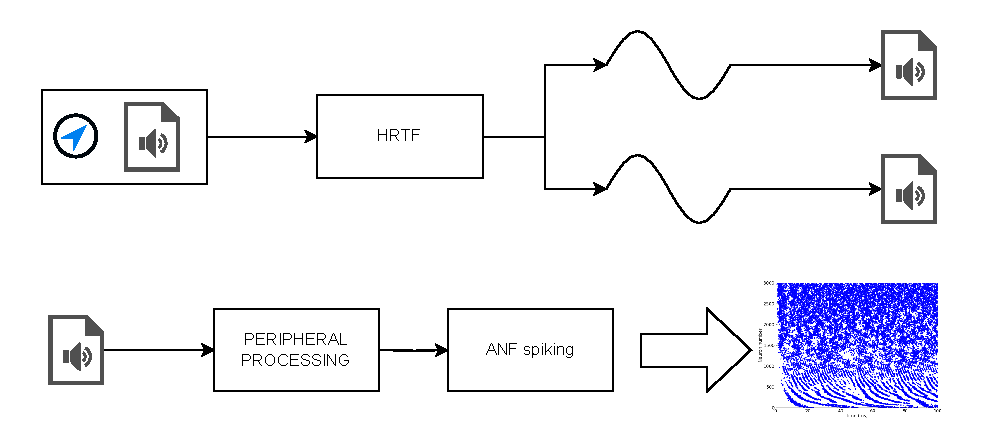
\includegraphics[width=1\linewidth]{Images/block-HRTF-cochlea-general.pdf}
        \caption{Block scheme for auditory peripheral processing}
        \label{fig:block-periph-general}
\end{figure}

\begin{figure}
    \centering
    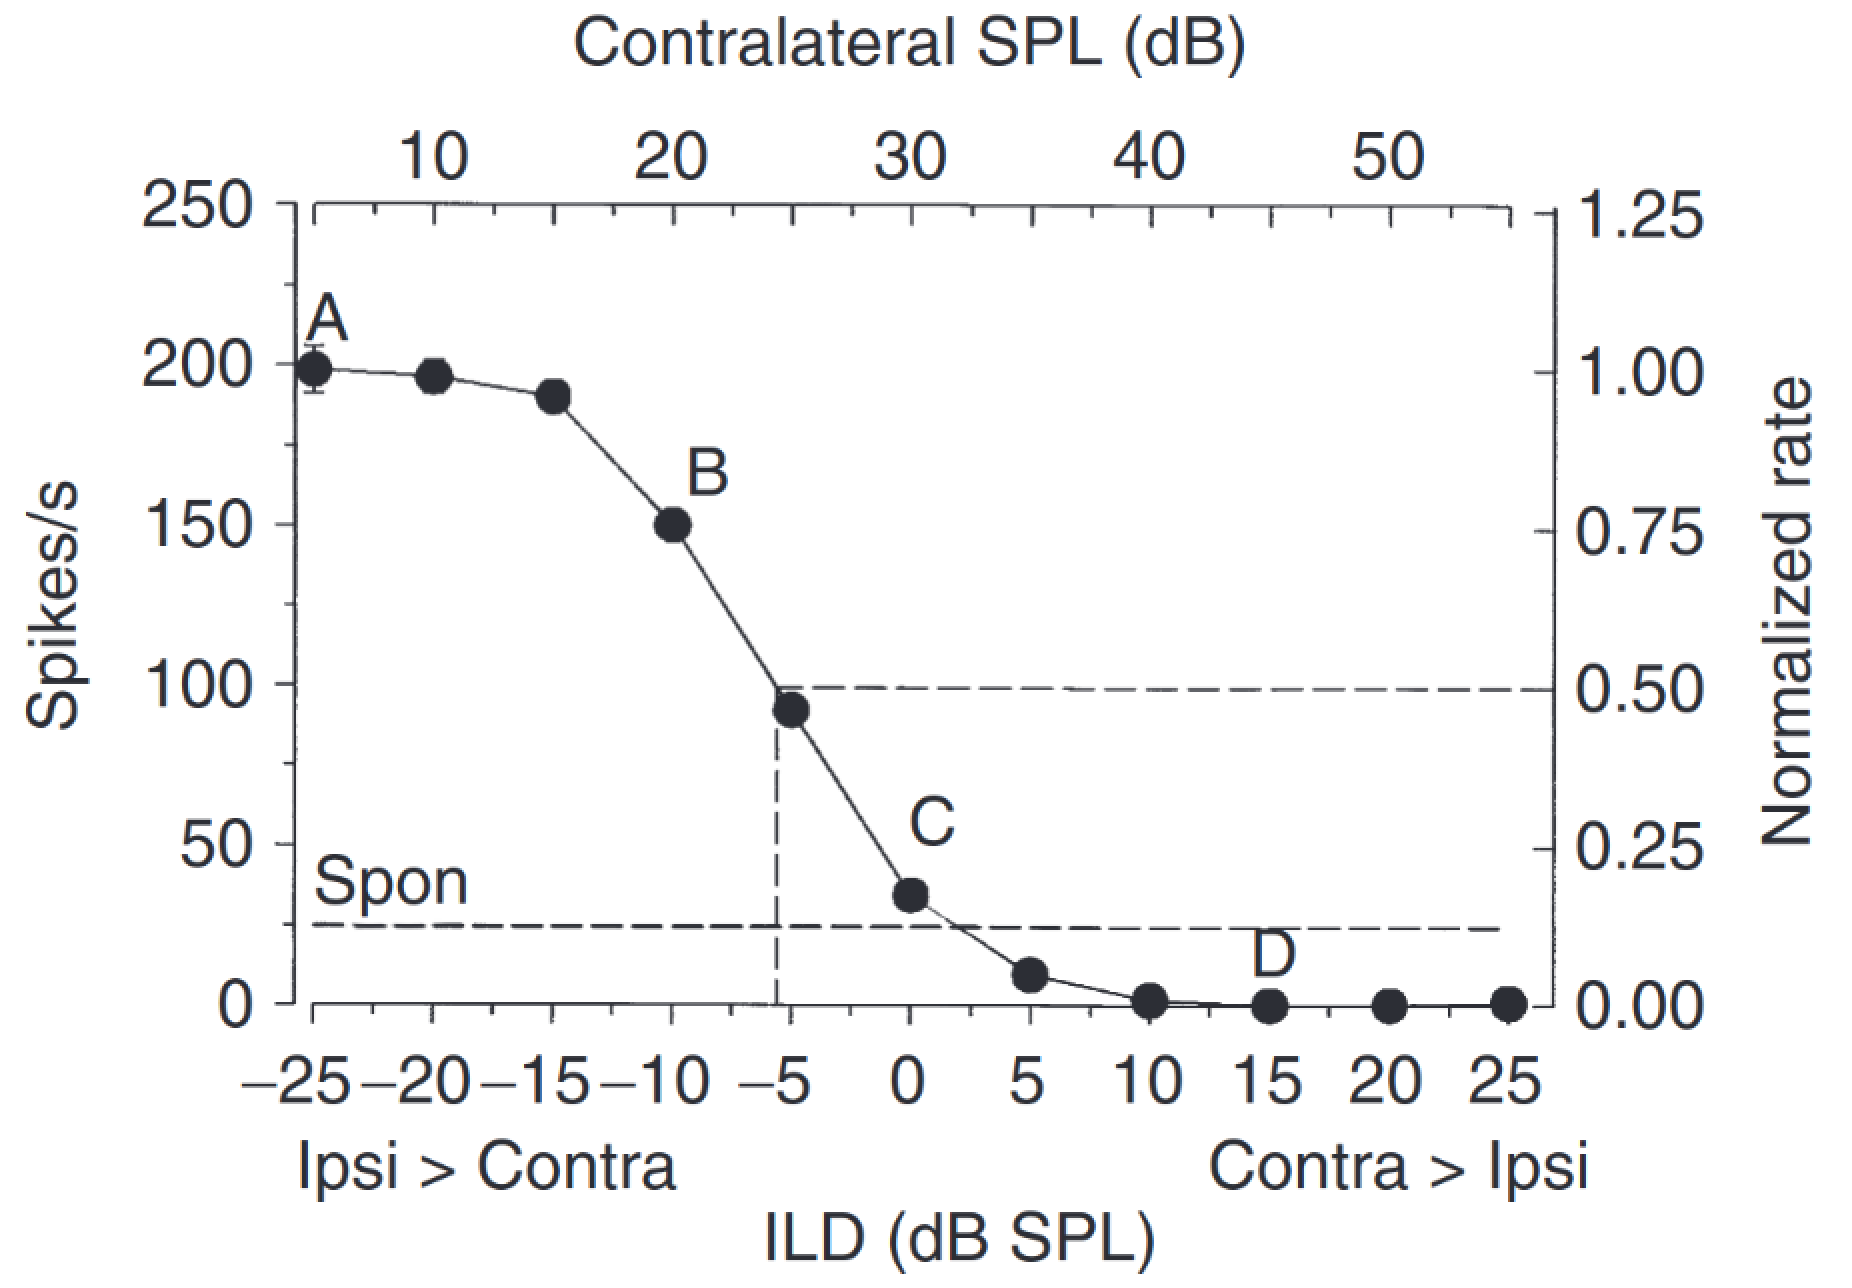
\includegraphics[width=0.7\linewidth]{Images/LSO-to-ILD.png}
    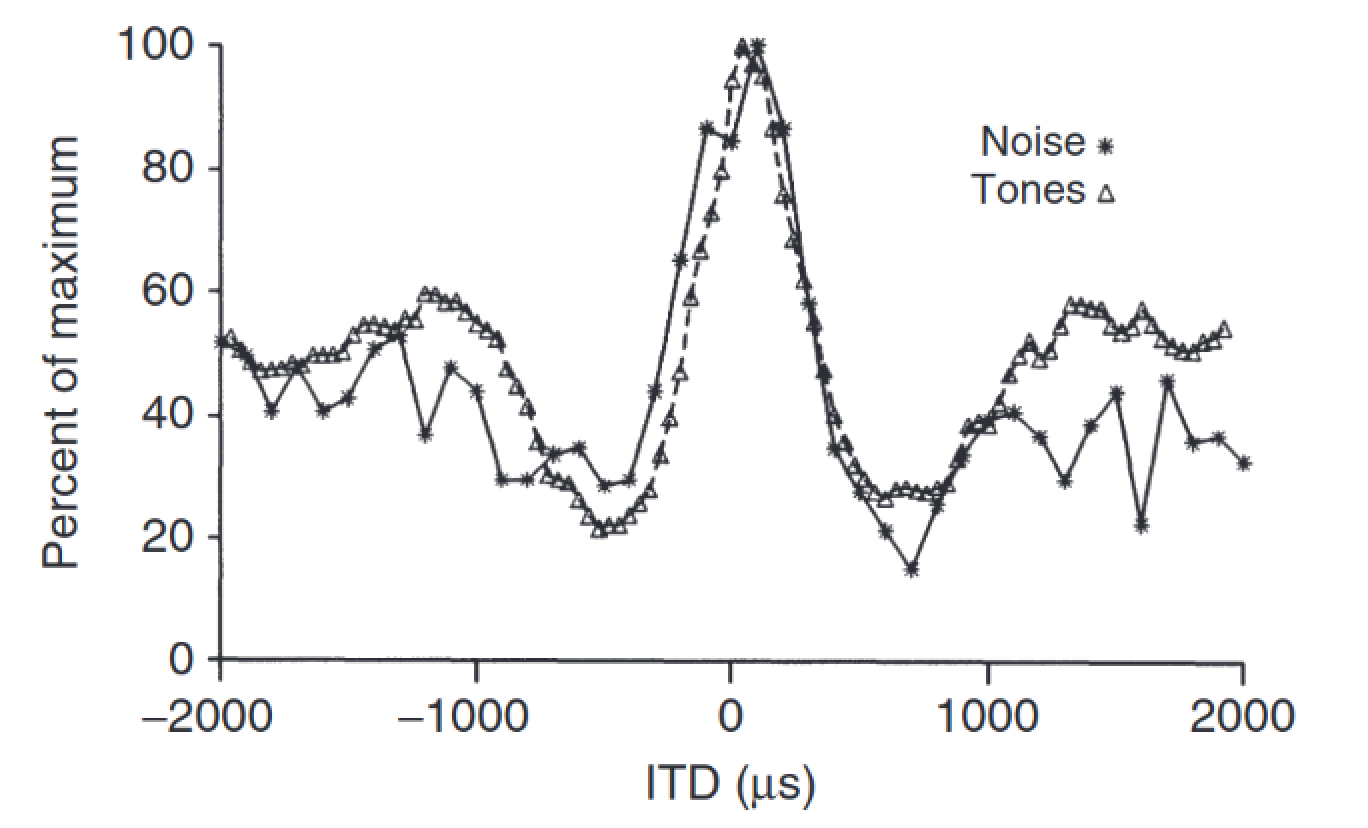
\includegraphics[width=0.7\linewidth]{Images/MSO-to-ITD.png}
    \caption{The response of SOC nuclei to the cue they are most sensitive to, adapted from \cite{yinNeuralMechanismsBinaural2019}. In the top plot, the response of an LSO cell to increasing contralateral level (increasing ILD). In the bottom plot, the response of an MSO cell to varying ITD. Notice the marked ipsilateral preference for the LSO, and contralateral-favoring response of the MSO.}
    \label{fig:lso-mso-expected}
\end{figure}

\subsection{IC}
Our last objective is to evaluate a possible way to combine cue processing by the LSO and the MSO. We draw a simple excitatory connection from both of them (the IC receives inputs from ipsilateral MSO and contralateral LSO), and we evaluate if the result improves compared to the LSO alone. To measure the \textit{improvement}, we computed the difference of the total population spikes between the two ICs for each azimuthal location. In the literature, the majority of IC neurons show ILD sensitivity, which would suggest a crucial role for the LSO in determining IC responses \cite{grotheMechanismsSoundLocalization2010}, and ILDs are the strongest cue for spatial tuning in the IC \cite{sleeLinearProcessingInteraural2013}. Because of this, we fit the difference in population activation to a LSO-like rate curve, described by a sigmoid with the following equation:
\begin{equation*}
    \frac{L}{1 + e^{-k(x - x_0)}} + b
\end{equation*}
We then define three metrics which will be the values that minimize non-linear least squares when applying the sigmoid to our data. The correspondence is as follows:
\begin{enumerate}
    \item \textit{$x_0$}: Closeness of center point to zero (to be minimized);
    \item \textit{$k$}: Steepness around zero (to be maximized);
    \item \textit{$L - b$}: Range, or the difference between maximum and minimum total population spike index (to be maximized).
\end{enumerate}
In addition, the $R^2$ value will tell us how well the difference in IC spike counts can be fit to the sigmoid.

\section{Results}
\subsection{Peripheral section}
We evaluated peripheral processing pathways based on the ANF response, focusing on vector strength (VS), a measure of phase synchrony, or how well spike timings are synchronized to a specific phase in each period. Some of our results are collected in Figure~\ref{fig:vectorstrength}, where we plot the phase responses, used to compute the VS, of a single ANF, one of the ten connected to the IHC. The selected ANF has an illustrative characteristic frequency (i.e., 500 Hz), receiving three-second tones with frequency 100 Hz, 500 Hz, and 5 kHz.

\begin{figure}
    \centering
    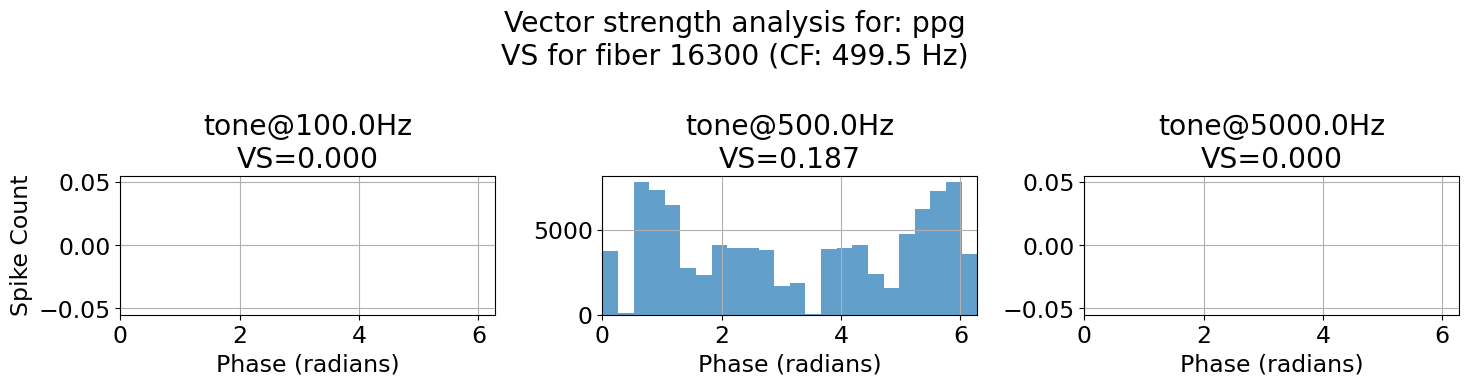
\includegraphics[width=1\linewidth]{Images/VSppg.png}
    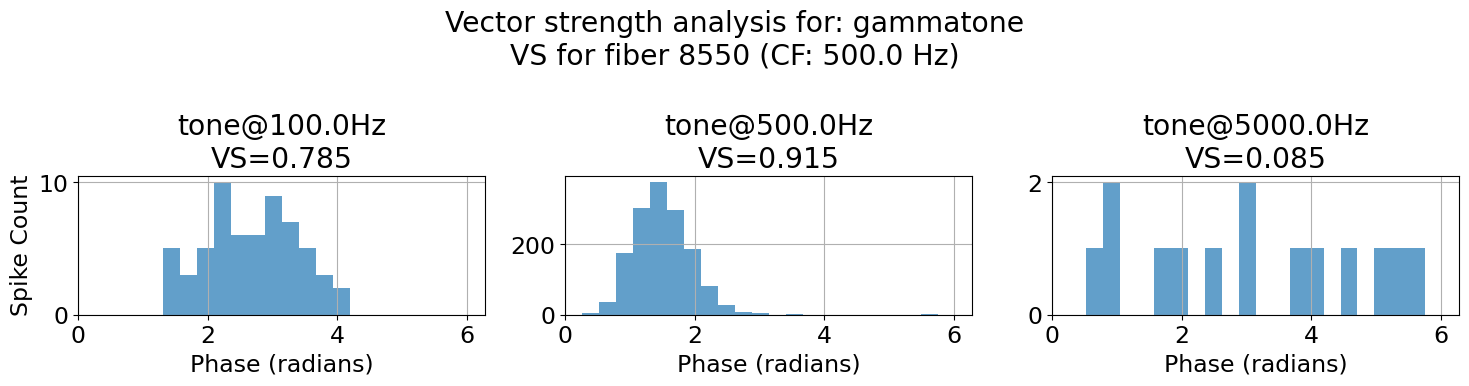
\includegraphics[width=1\linewidth]{Images/VSgamm.png}
    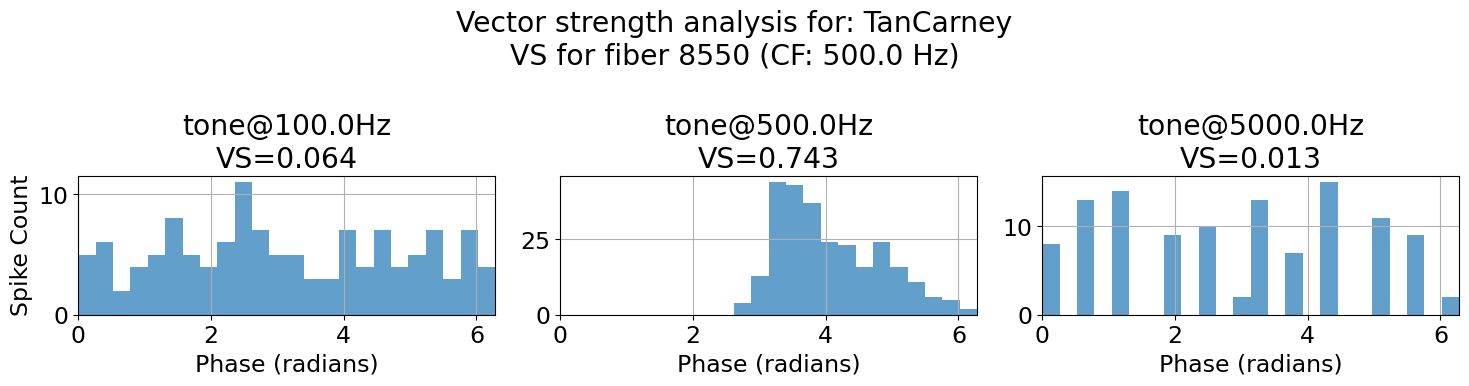
\includegraphics[width=1\linewidth]{Images/VStancarney.png}
    \caption{Each plot shows the vector strength and phase response of the same ANF in different peripheral processing pathways (in rows) and to different inputs (in columns, 100 Hz, 500 Hz, and 5 kHz).}
    \label{fig:vectorstrength}
\end{figure}

The results show that using more biologically plausible peripheral processing results in higher-quality ANF spike trains:
\begin{inlinelist}
    \item pulse packet generators were extremely faithful in tonotopic activation, as the only spiking ANFs are those in the immediate surrounding (a range of 2100 ANFs of the total 3500), which is in disagreement with both the gammatone-based and the Tan-Carney processing pathways
    \item the phase locking exhibited by the synthetic processing was very limited (VS = 0.187)
    \item\label{vs:gamm} the gammatone-based processing shows very accurate phase locking (VS = 0.915) for ANFs whose CFs were close to the input frequency, with a slow falloff for input frequencies further away from the CF (e.g., VS = 0.785 for a 100 Hz tone)
    \item the total number of spikes with gammatone-based processing is much higher than the most bioplausible version at CF, but falls off very quickly, possibly masking a lower phase locking than the one shown here
    \item the Tan-Carney-based processing shows a moderate VS for 500 Hz input (VS = 0.743) and lower spiking rates at CF, with respect to the gammatone 
    \item\label{vs:tclowfreq} in the Tan-Carney model, the 100 Hz input activates quite strongly, even if the CF is further away.
\end{inlinelist}
These findings show that both the gammatone-based and the Tan-Carney models present a sufficient level of bioplausibility for further processing. In addition, the Tan-Carney model shows higher vector strength (hence phase locking), more realistic spike counts with a less drastic falloff and some spontaneous rates, and more realistic falloff of ANF activation as the input tone frequency changes.


\subsection{Higher centers}
\paragraph{LSO}
In our testing, the behavior of the LSO was remarkably stable. Even when receiving input tones at low frequencies, for which the ILD is small as the attenuation given by the head is negligible, the sigmoidal shapes of left and right LSOs were unmistakable and very resistant to perturbations. The LSO remained consistent when we tried to change membrane time constants and connection weights. The typical dual sigmoidal response (see Fig\ref{fig:lso-mso-expected}) was also generated equally well by both realistic cochleas, as shown in \ref{fig:res-lso}. The difference between spike numbers of the two sides increased as frequency increased, as is to be expected with the rising ILD. When using the gammatone-based peripheral section, the LSO failed above \qty{10}{\kilo\hertz}. The vertical histograms show an additional difference between results: when using the gammatone-based peripheral section, the portion of population spiking (and contributing to the result) is very focused around the fibers with CF close to the input; instead, the Tan-Carney based results show more uniform activation of the entire population, with an increased spike rate for lower-frequency neurons.

\begin{figure*}
    \centering
    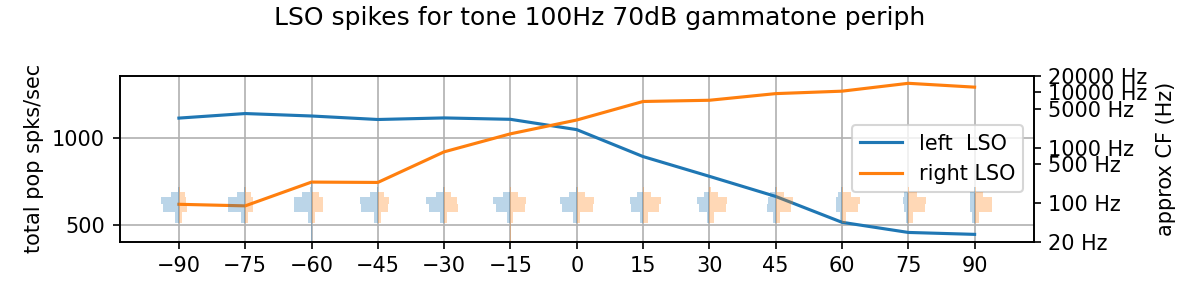
\includegraphics[width=0.4\linewidth]{Images/lso100.png}
    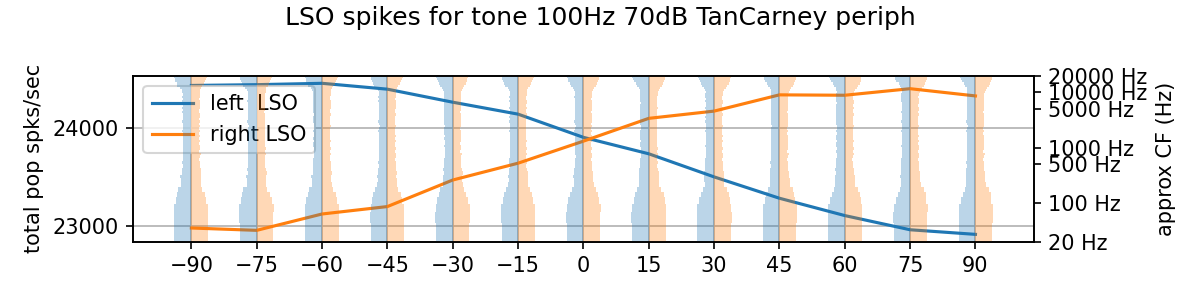
\includegraphics[width=0.4\linewidth]{Images/lso100tc.png}
    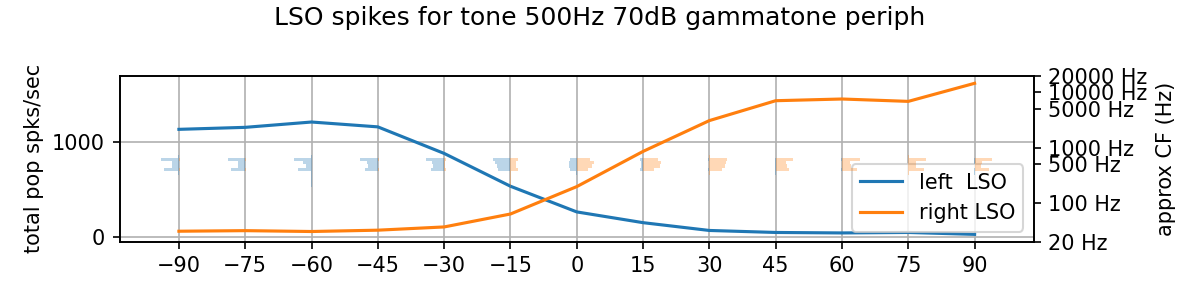
\includegraphics[width=0.4\linewidth]{Images/lso500.png}
    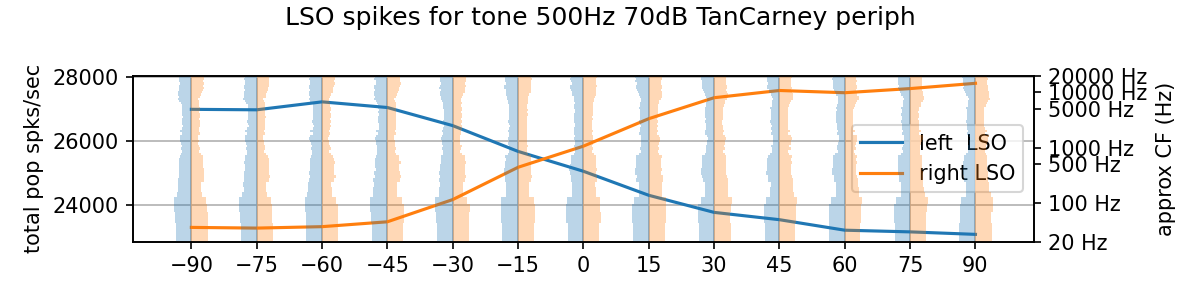
\includegraphics[width=0.4\linewidth]{Images/lso500tc.png}
    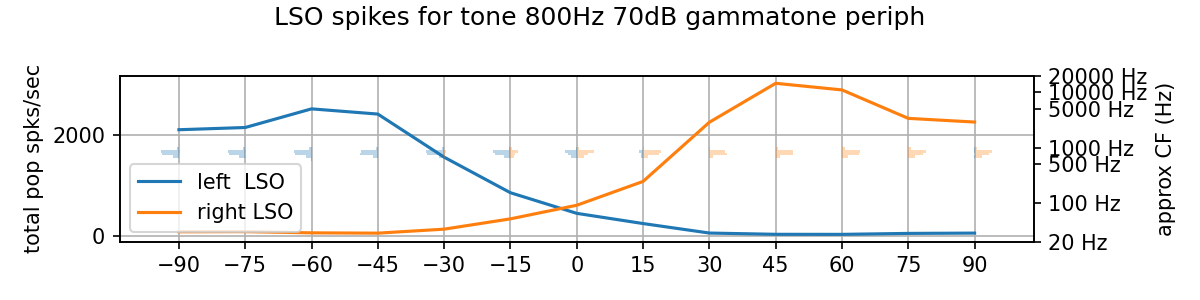
\includegraphics[width=0.4\linewidth]{Images/lso800.png}
    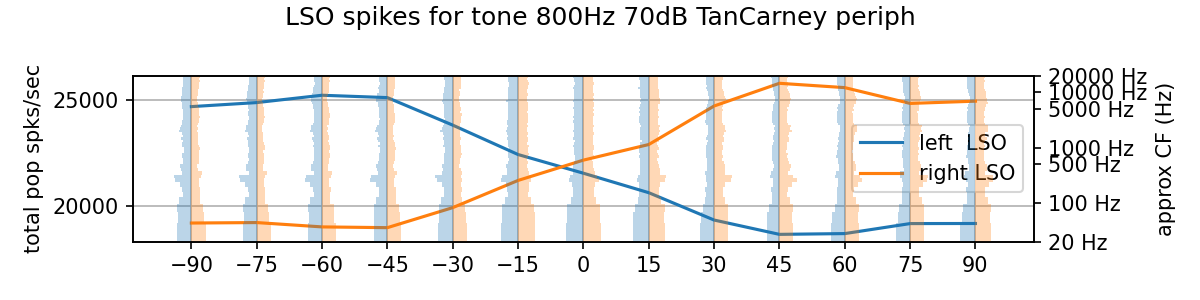
\includegraphics[width=0.4\linewidth]{Images/lso800tc.png}
    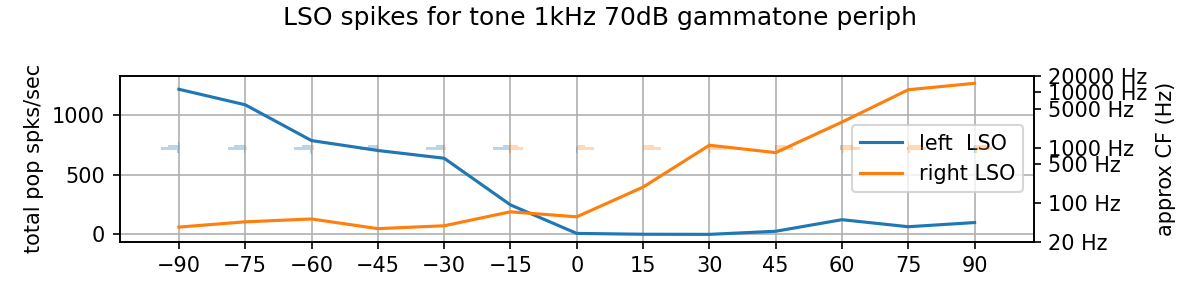
\includegraphics[width=0.4\linewidth]{Images/1khz.png}
    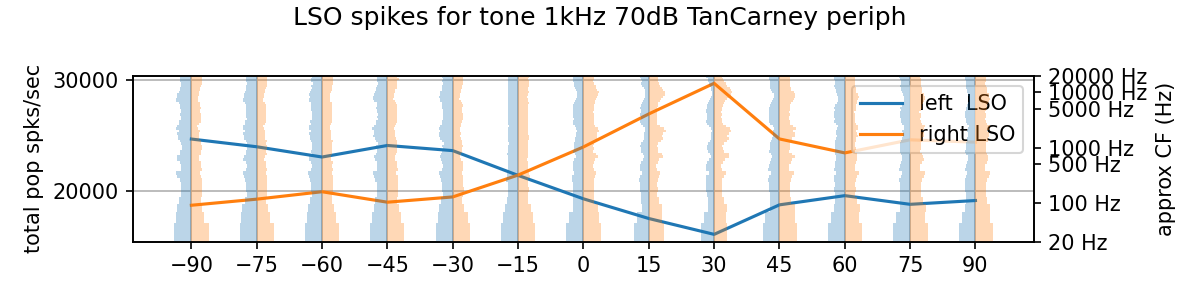
\includegraphics[width=0.4\linewidth]{Images/lso1000tc.png}
    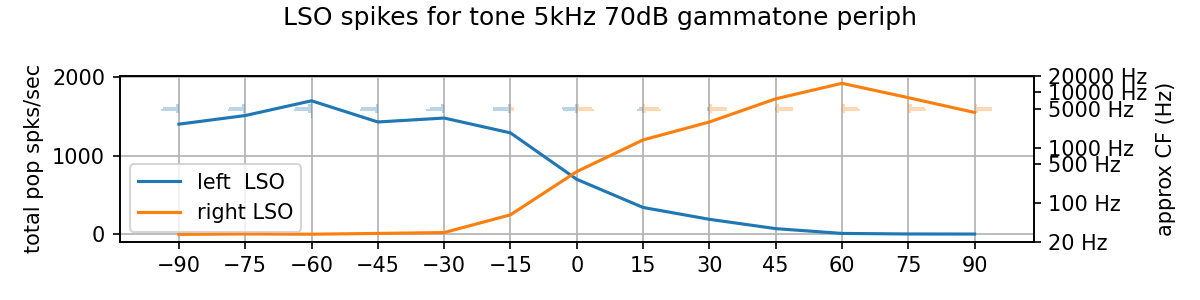
\includegraphics[width=0.4\linewidth]{Images/lso5khz.png}
    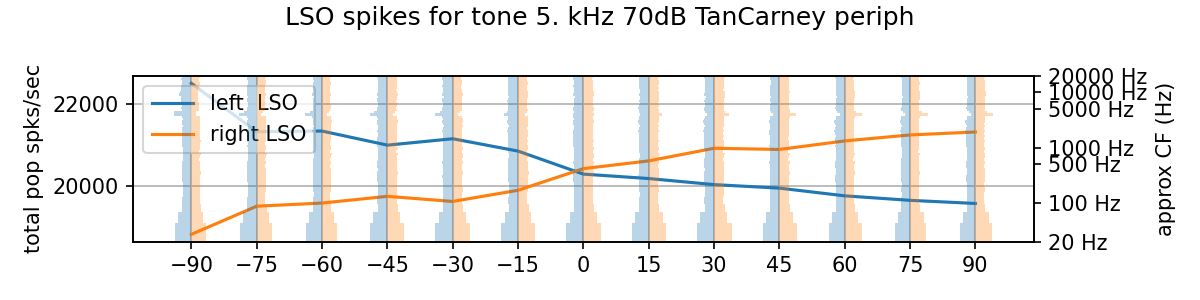
\includegraphics[width=0.4\linewidth]{Images/lso5000tc.png}
    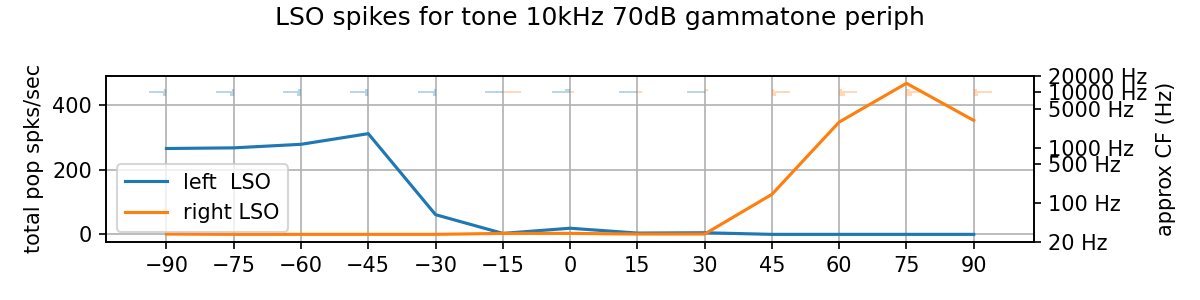
\includegraphics[width=0.4\linewidth]{Images/lso10khz.png}
    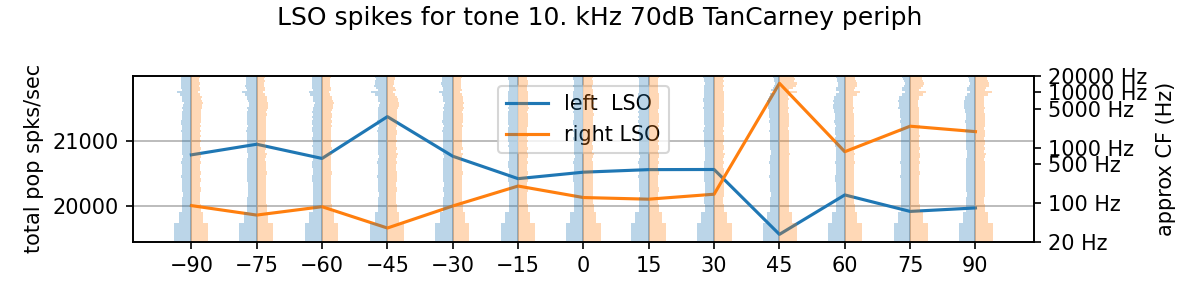
\includegraphics[width=0.4\linewidth]{Images/lso10000tc.png}
    \caption{Population spike rates for the LSO with growing frequencies, for gammatone-based (left) and Tan-Carney (right) processing.}
    \label{fig:res-lso}
\end{figure*}

\paragraph{MSO}
As with the LSO, the largest difference between the two bioplausible peripheral processing models is the extent of involved frequency ranges: while the gammatone-based processing only activates a narrow portion of ANFs (and hence the rest of the network), the Tan-Carney processing generates a broader activation. At the same time, MSO cells with high CF show a limited activation, possibly due to the slower decay time of inhibition, which, at high frequencies, stops cells almost completely. Decay with rising frequency is not the same between the two input sources: while the gammatone-based falls off quickly, losing differentiating abilities at \qty{800}{\hertz}, the Tan-Carney-based shows higher spiking rates at contralateral angles also at \qty{10}{\kilo\hertz}.
\begin{figure*}
    \centering
    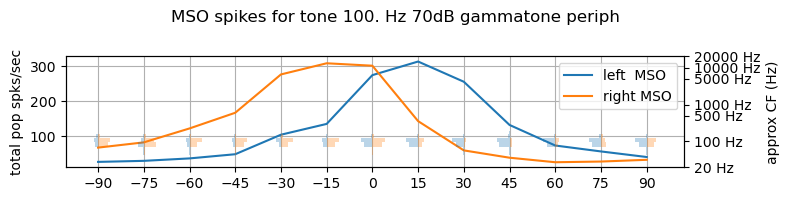
\includegraphics[width=0.4\linewidth]{Images/gamm100.png}
    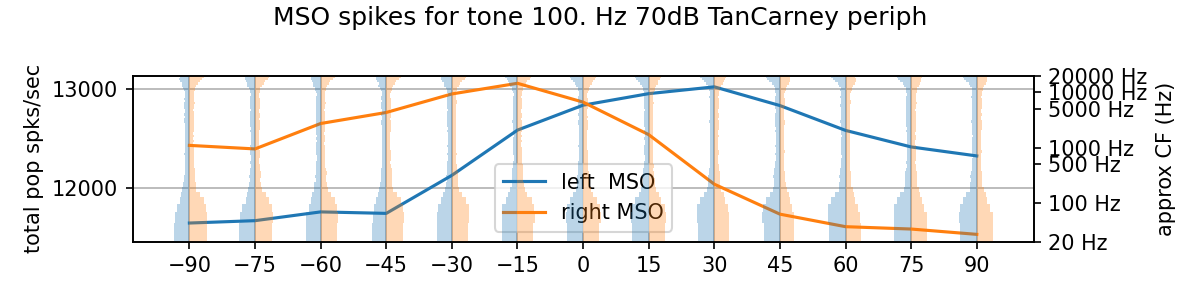
\includegraphics[width=0.4\linewidth]{Images/mtc100.png}
    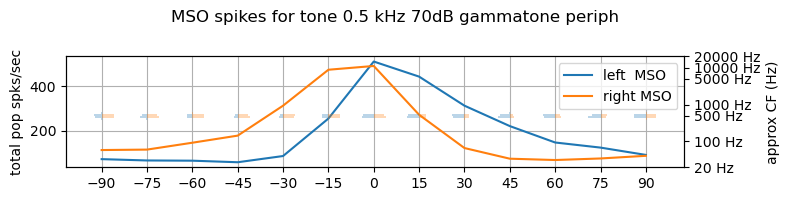
\includegraphics[width=0.4\linewidth]{Images/gamm500.png}
    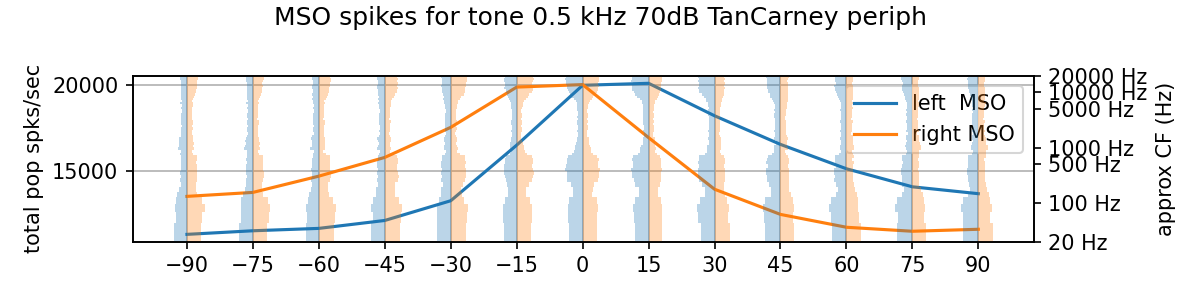
\includegraphics[width=0.4\linewidth]{Images/mtc500.png}
    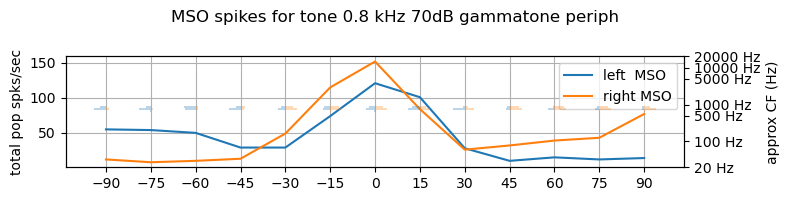
\includegraphics[width=0.4\linewidth]{Images/gamm800.png}
    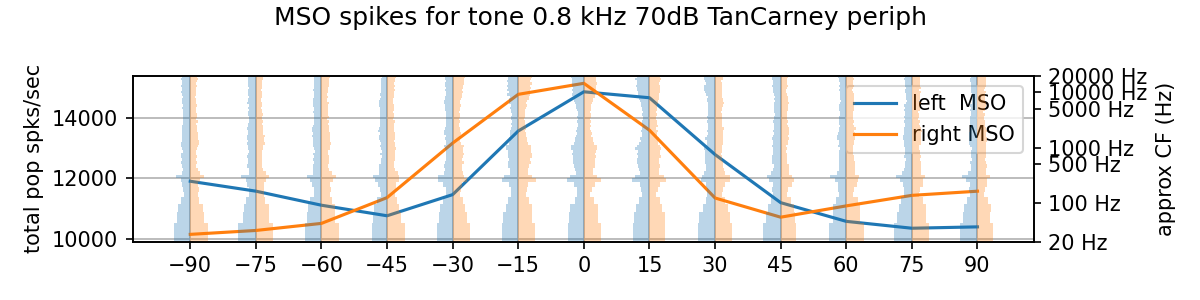
\includegraphics[width=0.4\linewidth]{Images/mtc800.png}
    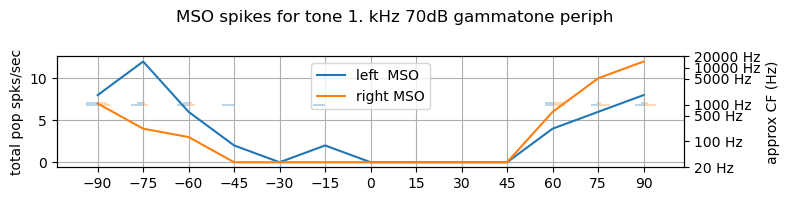
\includegraphics[width=0.4\linewidth]{Images/gamm1000.png}
    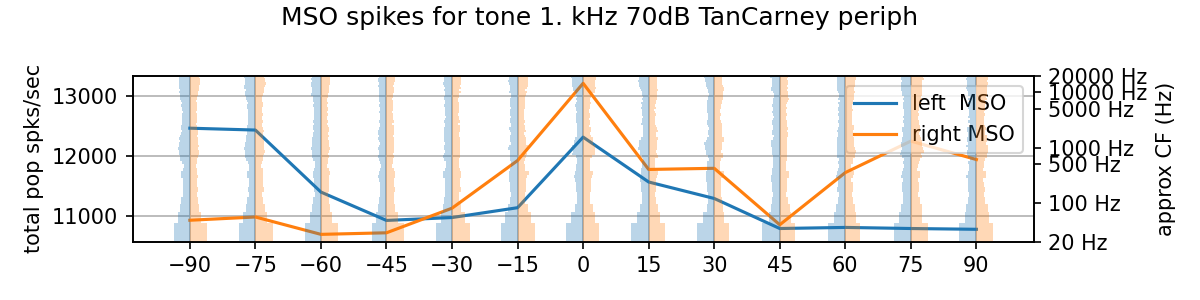
\includegraphics[width=0.4\linewidth]{Images/mtc1000.png}
    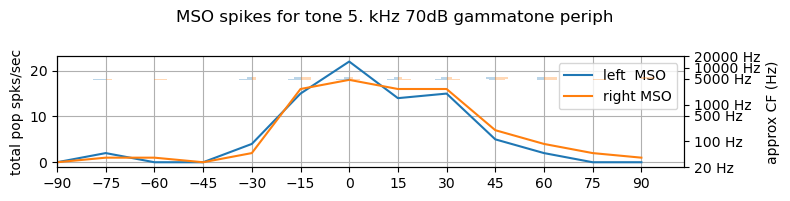
\includegraphics[width=0.4\linewidth]{Images/gamm5000.png}
    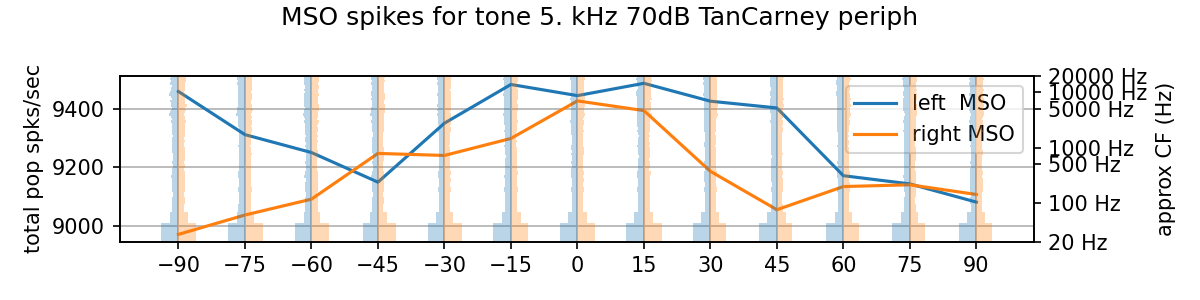
\includegraphics[width=0.4\linewidth]{Images/mtc5000.png}
    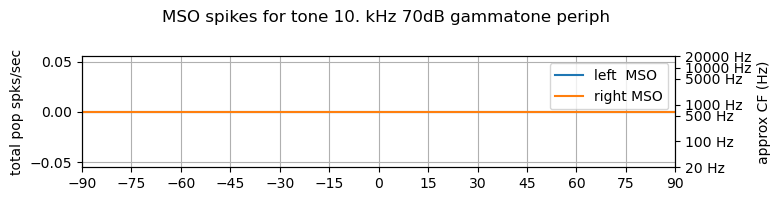
\includegraphics[width=0.4\linewidth]{Images/gamm10000.png}
    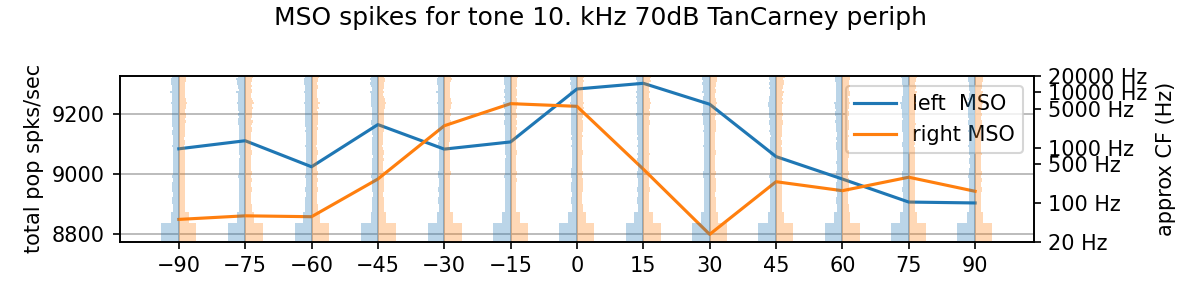
\includegraphics[width=0.4\linewidth]{Images/mtc10000.png}
    \caption{Population spike rates for the MSO with growing frequencies, for gammatone-based (left) and Tan-Carney (right) processing.}
    \label{fig:res-mso}
\end{figure*}

Although the impact of the contralateral preference is limited, MSO behavior shows that Myoga's principles to influence coincidence detection are applicable. This warrants additional research, focused on verifying whether it is possible to fully replicate MSO recordings in larger animals using differences in arrival times of inhibition and excitation, without dedicated delay lines or other, less bioplausible interactions.

\subsection{Inferior Colliculus}
Finally, we consider whether the integration of cues from MSO and LSO proved beneficial to the IC. To determine the impact of the MSO on the IC curves, we focus on the most bioplausible version of our peripheral processing (i.e., the Tan-Carney model). In Figure~\ref{fig:lso-icc-fit-sigmoid}, we plot the difference of total population spikes between the right and left LSO (top) and IC (bottom). Note that the IC integrates the input of the contralateral LSO and ipsilateral MSO. The results are not particularly striking: while the steepness around the center point improved, this came at a cost for range, which decreased in the IC compared to the LSO. Overall, the zero crossing accuracy was the most significant improvement, which at low frequencies was improved significantly. At the same time, due to database constraints, our data points are 15 degrees apart, and even the largest improvement in zero crossing was by around 3 degrees.     

\begin{figure*}
    \centering
    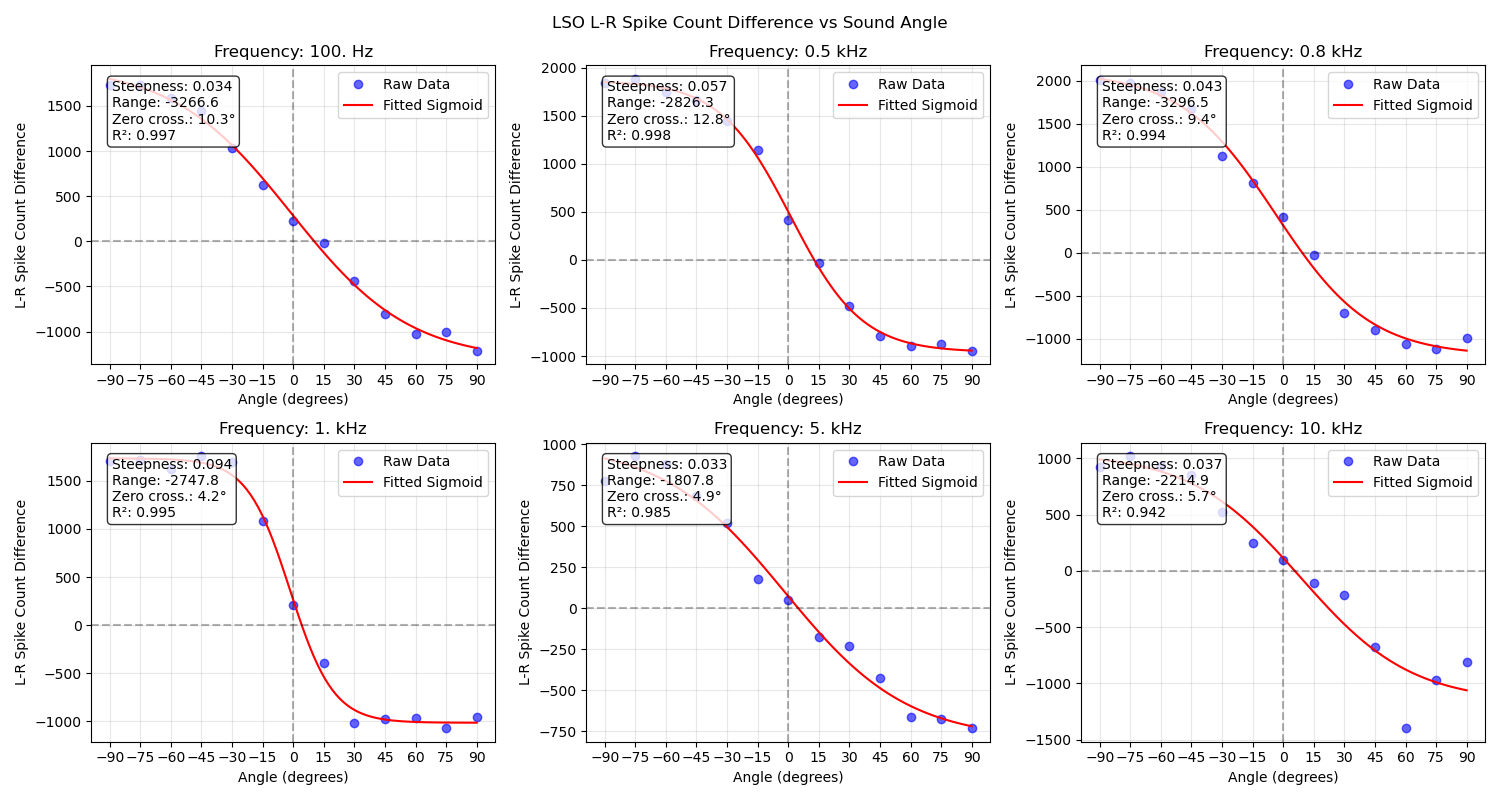
\includegraphics[width=0.7\linewidth]{Images/LSOfit.png}
    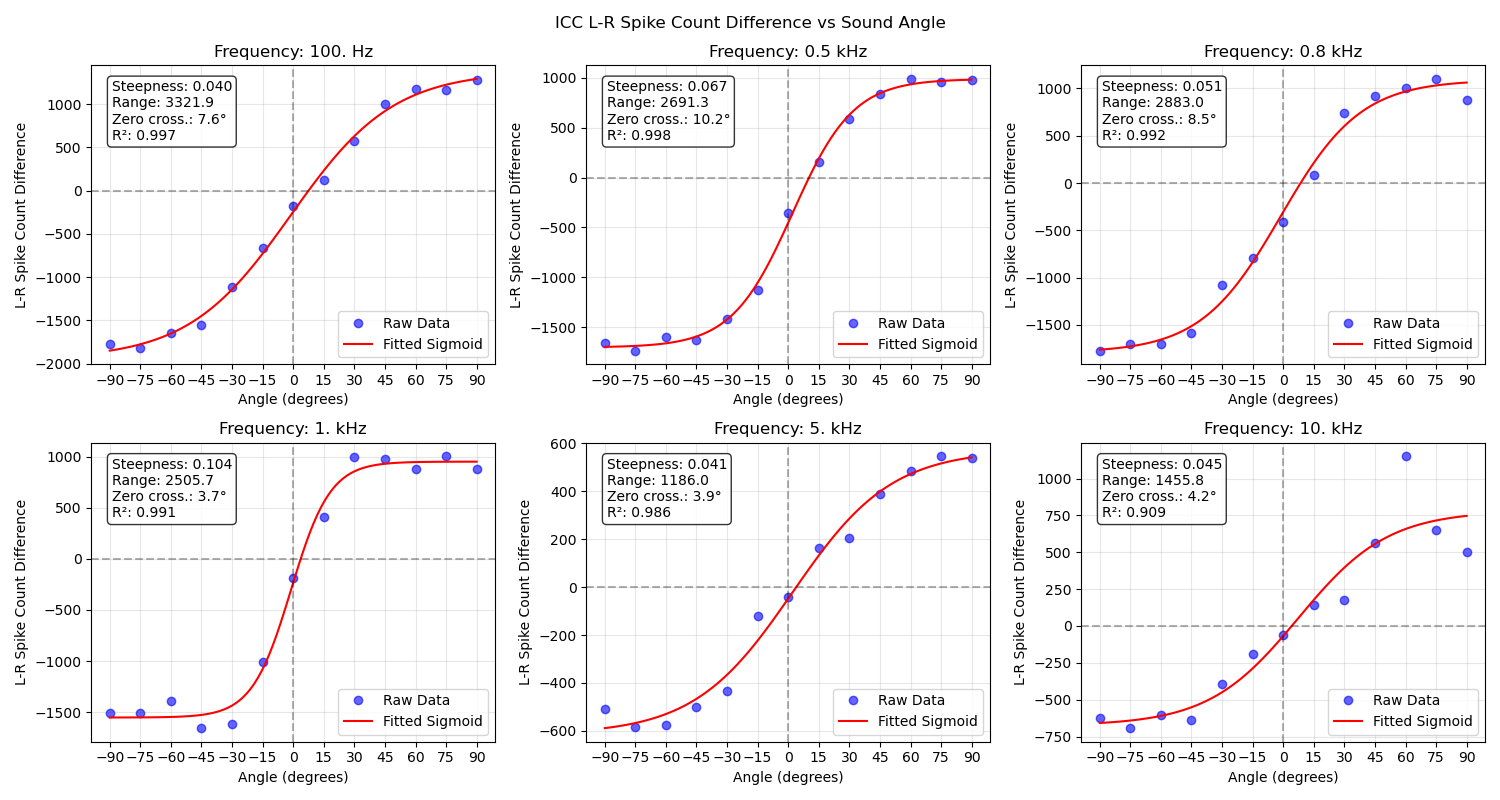
\includegraphics[width=0.7\linewidth]{Images/ICCfit.png}
    \caption{Comparison of sigmoid fit for all frequencies. Top: LSO. Bottom: IC. Because the contralateral LSO connects to IC, its slope is in the opposite direction.}
    \label{fig:lso-icc-fit-sigmoid}
\end{figure*}


\section{Conclusions}
With this work, we have shown evidence for three claims: 
\begin{inlinelist}
    \item bioplausible peripheral processing achieves ANF spiking patterns that contain fundamental information for localization (as seen with the phase response);
    \item using Myoga's principles for a bioplausible MSO results in a contralateral-favoring MSO;
    \item we were unable to find a significant improvement in the IC response curves when using a simple excitatory-excitatory connection scheme with the SOC nuclei.
\end{inlinelist}


%---------------------------------------------------------------------------
%  BIBLIOGRAPHY
%---------------------------------------------------------------------------
% Remember to insert here only the essential bibliography of your work
\bibliography{bibliography.bib} % automatically inserted and ordered with this command 

\end{document}